\documentclass{beamer}
\usepackage[utf8]{inputenc}
\usepackage{graphicx}
\usepackage{xcolor}
\usetheme{default}
\usecolortheme{default}

\title[S02 Régression et MCO]{Section 02 : Régression et Moindres Carrés Ordinaires\\ (Application Stata)}
\subtitle{GSF-6053: Économétrie Financière}
\author[SP. Boucher]{Simon-Pierre Boucher\inst{1}}
\institute[Université Laval]
{
  \inst{1}%
  Département de finance, assurance et immobilier\\
  Faculté des sciences de l'administration\\
  Université Laval}
\date[Hiver 2022]{1 Février 2022}

\begin{document}

\begin{frame}
  \titlepage
\end{frame}

\begin{frame}{Application STATA}
\begin{itemize}
\item Dans cette application Stata, nous allons analyser le jeu de données portant le nom \textbf{Wage1}
\item Il s’agit essentiellement de données collectées auprès de plusieurs travailleurs en 1976.
\item Dans cette analyse nous chercherons à quantifier et expliquer l’impact de certains facteurs propre au salarié sur son salaire.
\item Les variables que nous utiliserons dans cette analyse sont les suivantes:
\begin{itemize}
\item \textbf{lwage:} log du salaire horaire moyen
\item \textbf{educ:} années d'études
\item \textbf{exper:} années d'expérience potentielle
\item \textbf{tenutre:} années chez l'employeur actuel
\end{itemize}
\end{itemize}
\end{frame}

\begin{frame}{Application STATA}

\begin{block}{Code 1: Pour obtenir jeu de données Wage1 sur Stata}
\textbf{use http://fmwww.bc.edu/ec-p/data/wooldridge/wage1}
\end{block}

\begin{block}{Code 2: Vérifier le format des variables utilisées}
\textbf{describe wage educ exper tenure}
\end{block}

\begin{block}{Output 2:}
\begin{center}
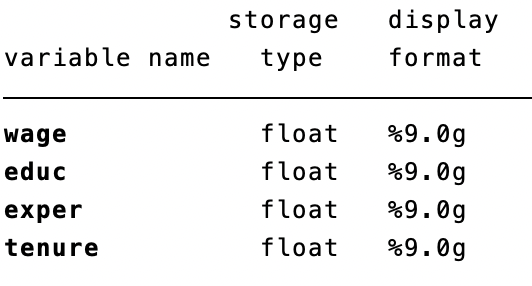
\includegraphics[scale=.5]{describe}
\end{center}
\begin{itemize}
\item On peut voir que nos trois variables sont de type Float, ce qui indique qu'il s'agit d'une valeur numérique entière. 
\item On peut donc l'utiliser pour notre analyse.
\end{itemize}
\end{block}

\end{frame}


\begin{frame}{Application STATA}
\begin{block}{Code 3: Calculer et afficher des statistiques descriptives}
\textbf{summarize wage educ exper tenurex}
\end{block}
\begin{block}{Output 3:}
\begin{center}
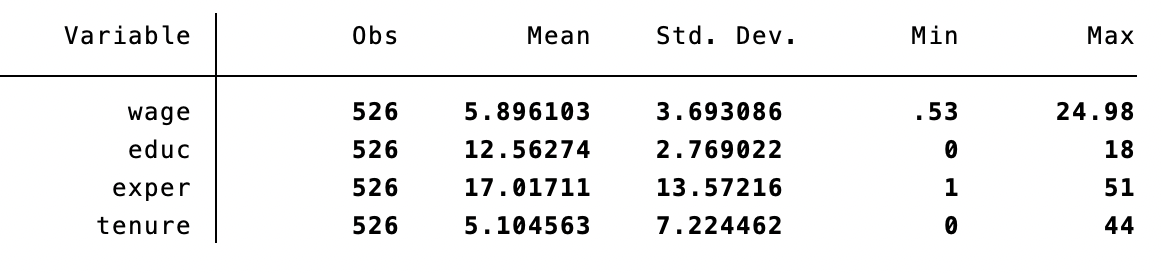
\includegraphics[scale=.5]{summary}
\end{center}
\begin{itemize}
 \item On peut voir que notre jeu de données contient 526  observations 
 \item Que le salaire moyen horraire est de 5.89 et qu'en moyenne les salariés ont 12.56 années de scolarité. 
 \item Pour ce qui est de l'expérience de travail, en moyenne les salariés ont 17.02 années d'expériences et ils sont dans le même emploie depuis 5.10 ans, en moyenne.
\end{itemize}
\end{block}

\end{frame}


\begin{frame}{Application STATA}
\begin{block}{Code 4: Relation entre le salaire et l'éducation}
\textbf{twoway (scatter wage educ) (lfit wage educ)}
\end{block}

\begin{block}{Output 4:}
\begin{center}
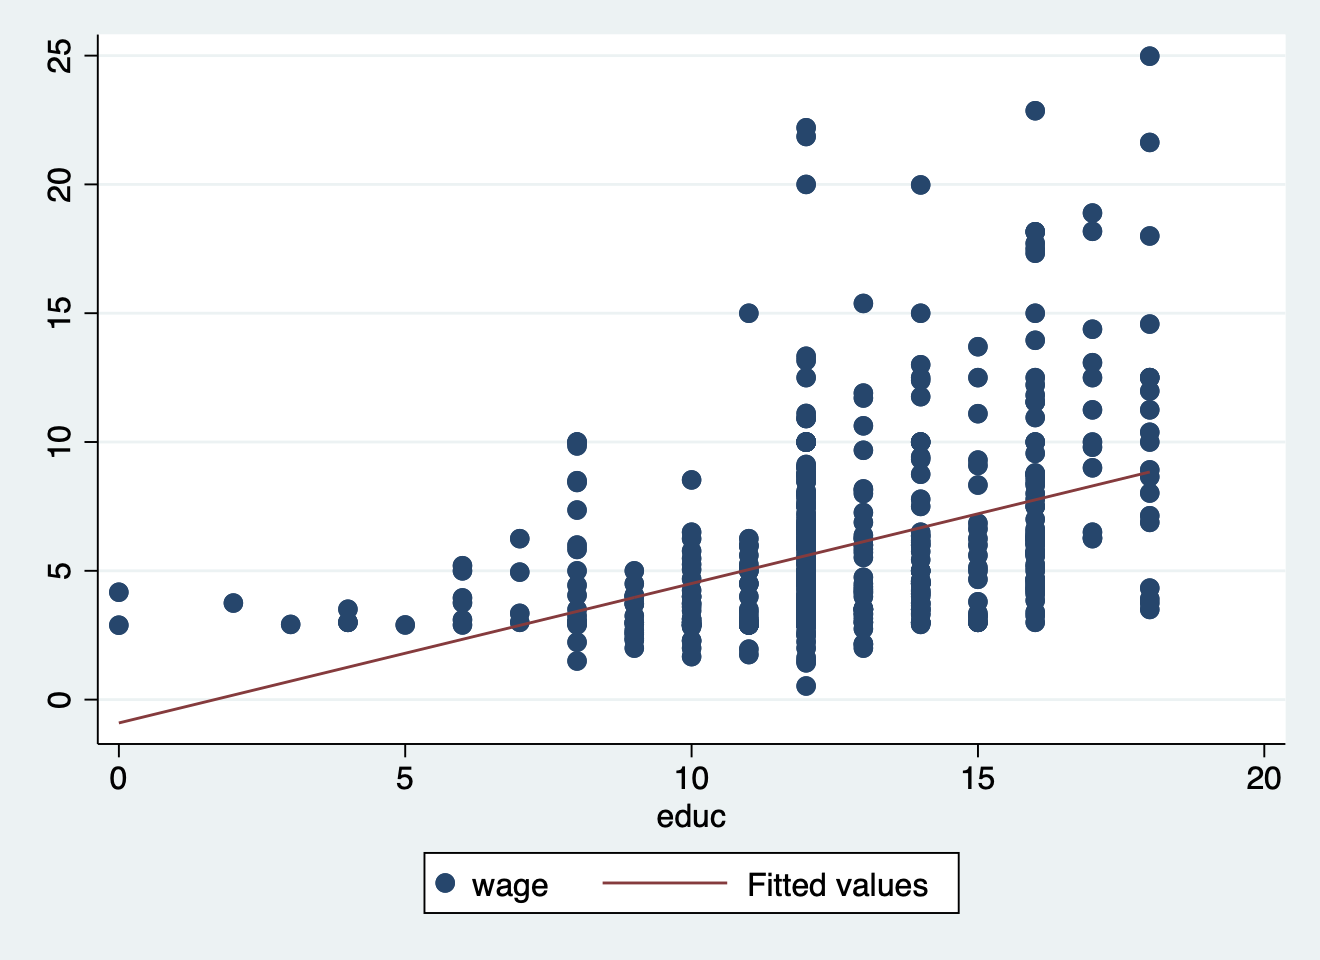
\includegraphics[scale=.3]{PLOT_1.png}
\end{center}
\end{block}
\end{frame}


\begin{frame}{Application STATA}
\begin{block}{Code 5: Relation entre le salaire et l'expérience de travail}
\textbf{twoway (scatter wage exper) (lfit wage exper)}
\end{block}

\begin{block}{Output 5:}
\begin{center}
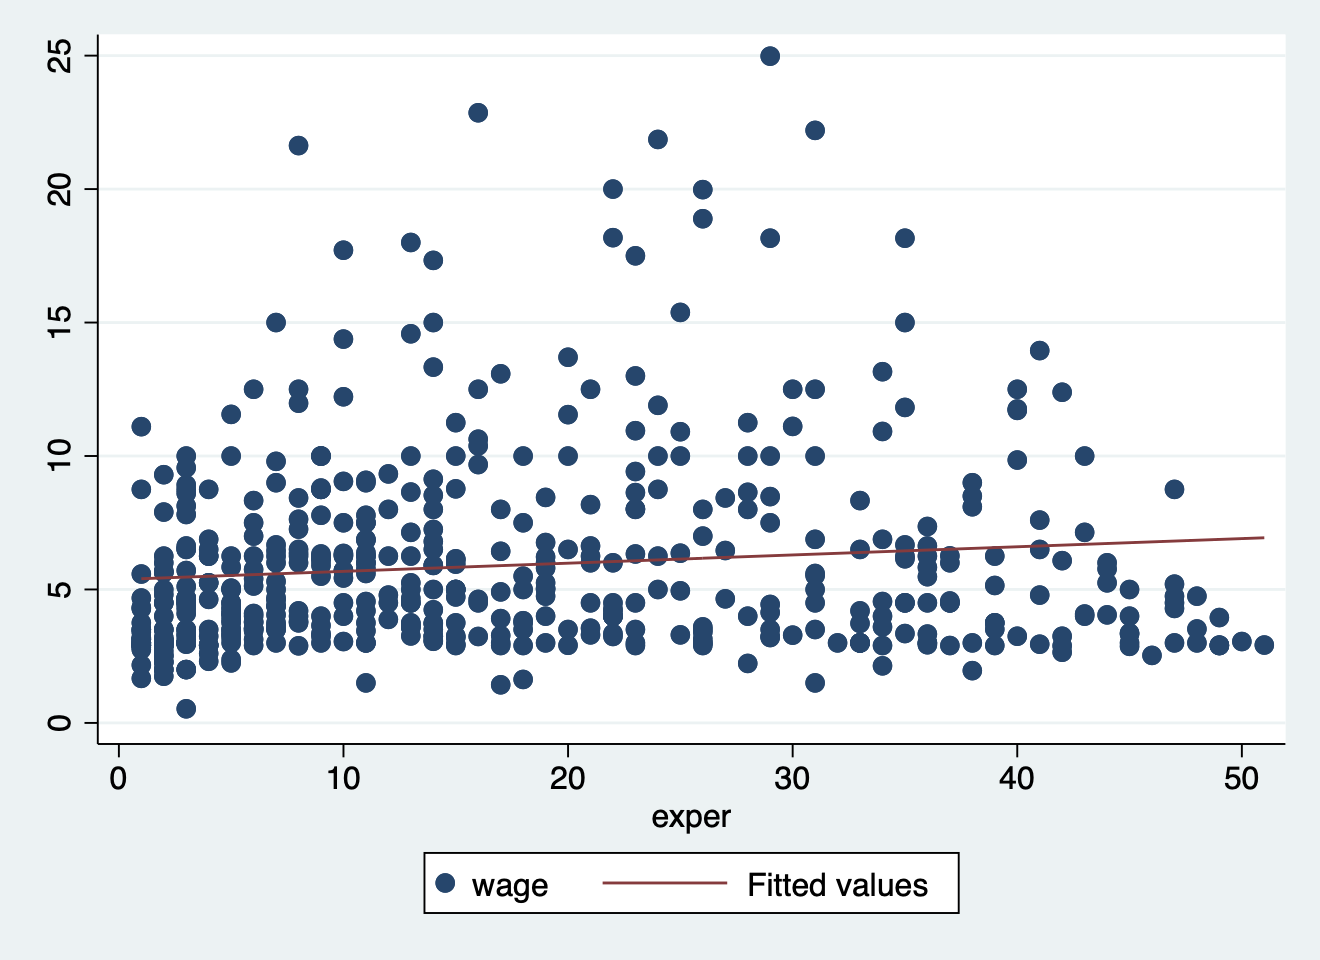
\includegraphics[scale=.3]{PLOT_2.png}
\end{center}
\end{block}
\end{frame}

\begin{frame}{Application STATA}
\begin{block}{Code 6: Relation entre le salaire et le nombre d'années chez l'employeur actuel}
\textbf{twoway (scatter wage tenure) (lfit wage tenure)}
\end{block}

\begin{block}{Output 6:}
\begin{center}
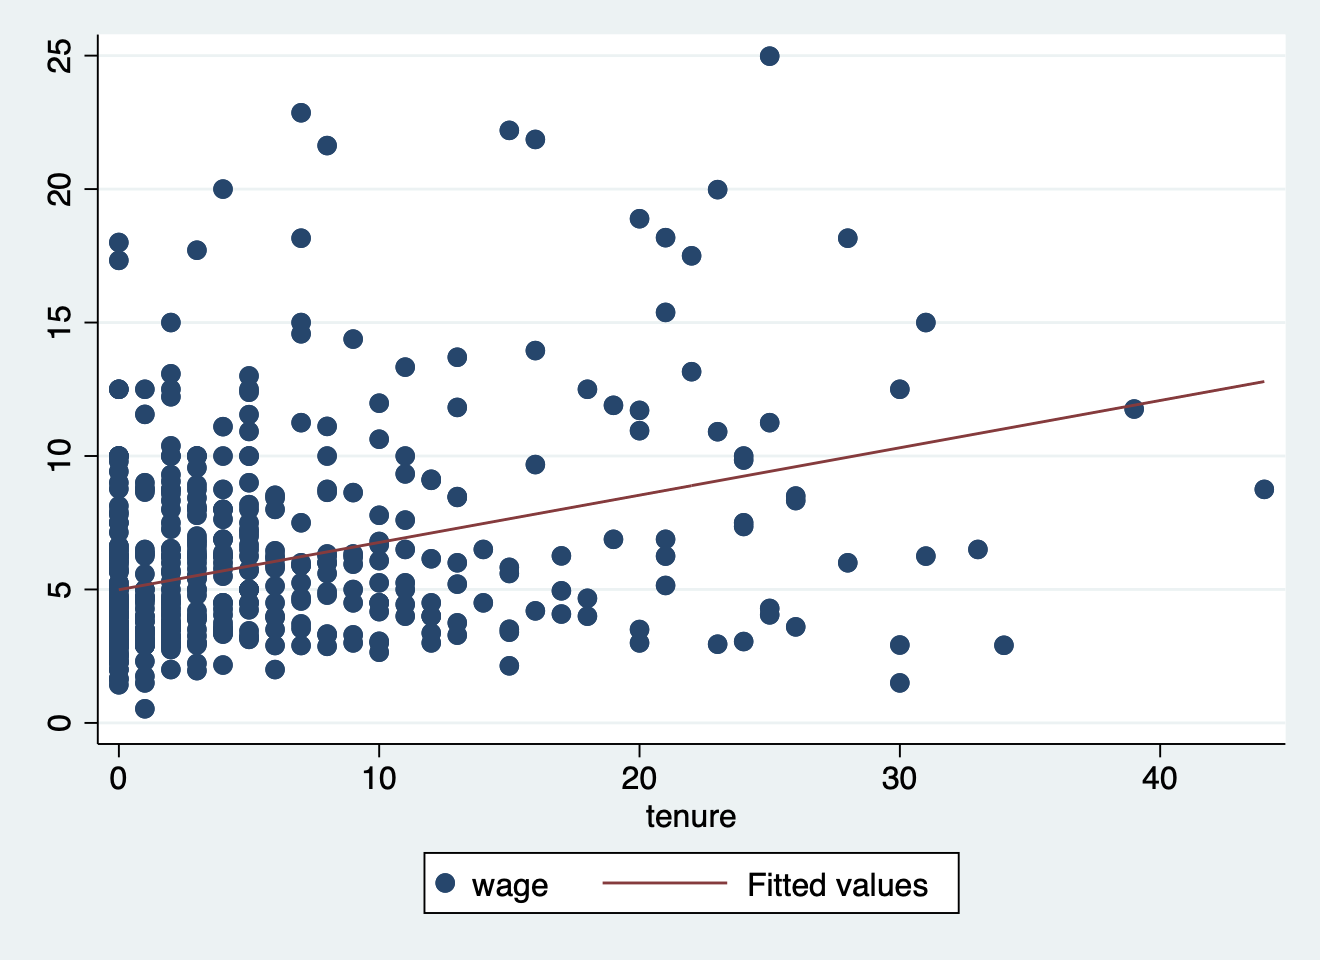
\includegraphics[scale=.3]{PLOT_3.png}
\end{center}
\end{block}
\end{frame}

\begin{frame}{Application STATA}
\begin{block}{Code 7: Distrbution de la variable \textbf{wage}}
\textbf{histogram wage, bin(50) normal normopts(lwidth(thick))}
\end{block}

\begin{block}{Output 7:}
\begin{center}
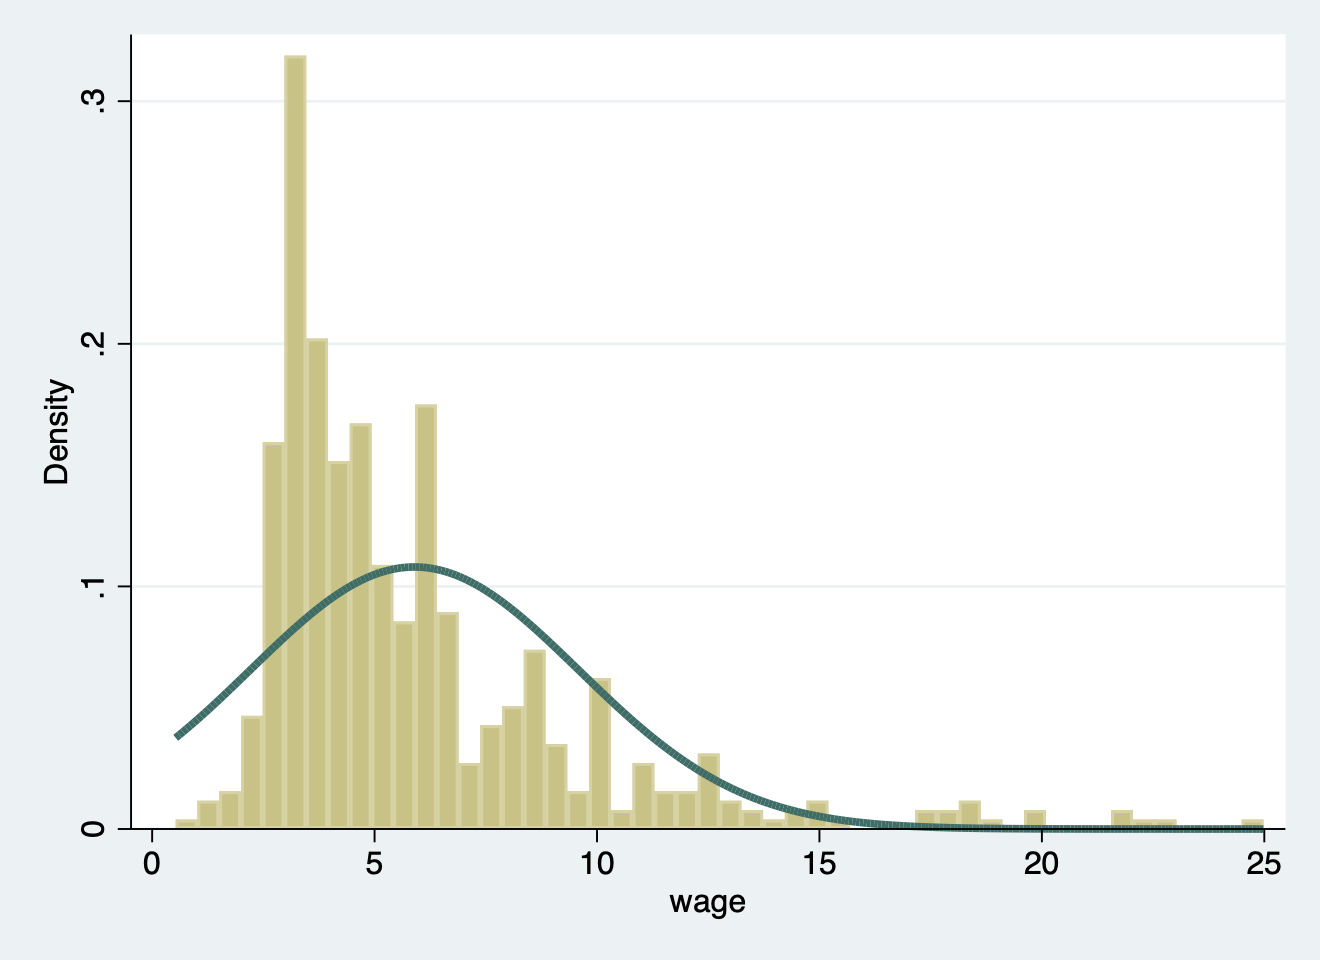
\includegraphics[scale=.3]{PLOT_4.png}
\end{center}
\end{block}
\end{frame}

\begin{frame}{Application STATA}
\begin{block}{Code 8: Distrbution de la variable \textbf{educ}}
\textbf{histogram educ, bin(20) normal normopts(lwidth(thick))}
\end{block}

\begin{block}{Output 8:}
\begin{center}
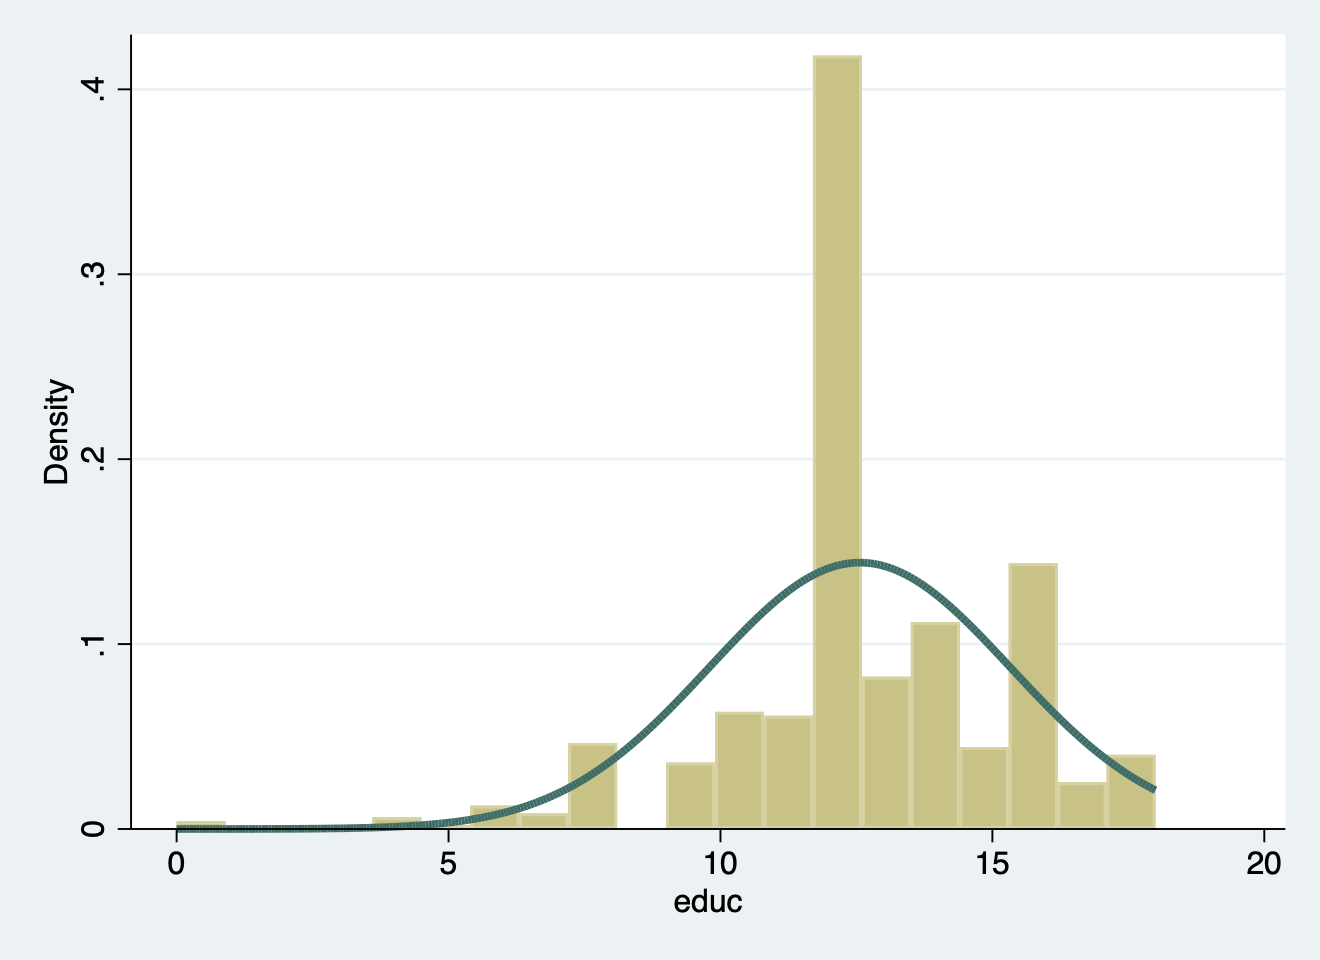
\includegraphics[scale=.3]{PLOT_5.png}
\end{center}
\end{block}
\end{frame}


\begin{frame}{Application STATA}
\begin{block}{Code 9: Distrbution de la variable \textbf{exper}}
\textbf{histogram exper, bin(50) normal normopts(lwidth(thick))}
\end{block}

\begin{block}{Output 9:}
\begin{center}
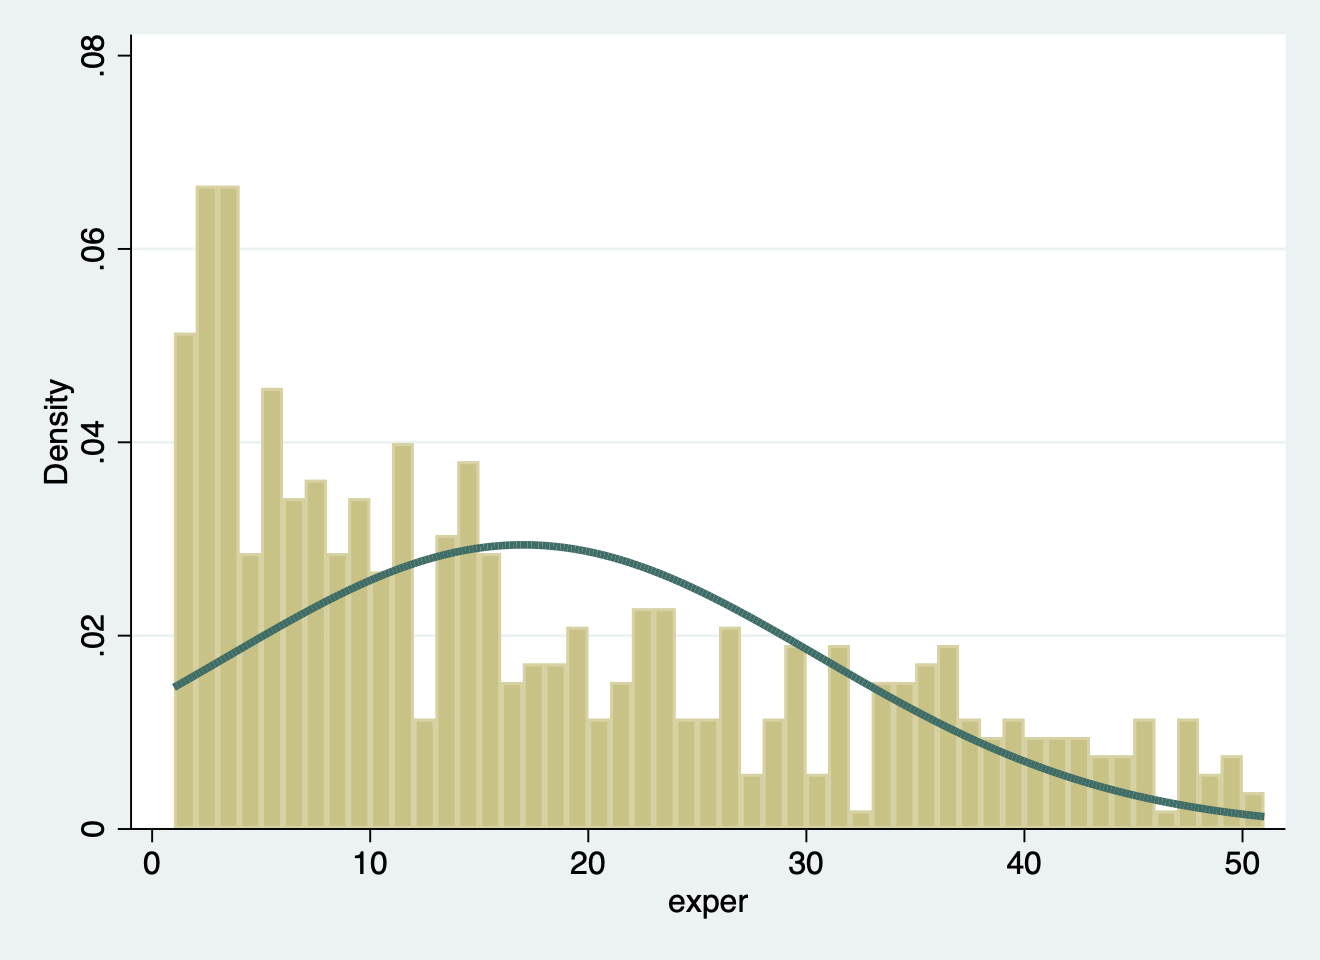
\includegraphics[scale=.3]{PLOT_6.png}
\end{center}
\end{block}
\end{frame}

\begin{frame}{Application STATA}
\begin{block}{Code 10: Distrbution de la variable \textbf{tenure}}
\textbf{histogram tenure, bin(30) normal normopts(lwidth(thick))}
\end{block}

\begin{block}{Output 10:}
\begin{center}
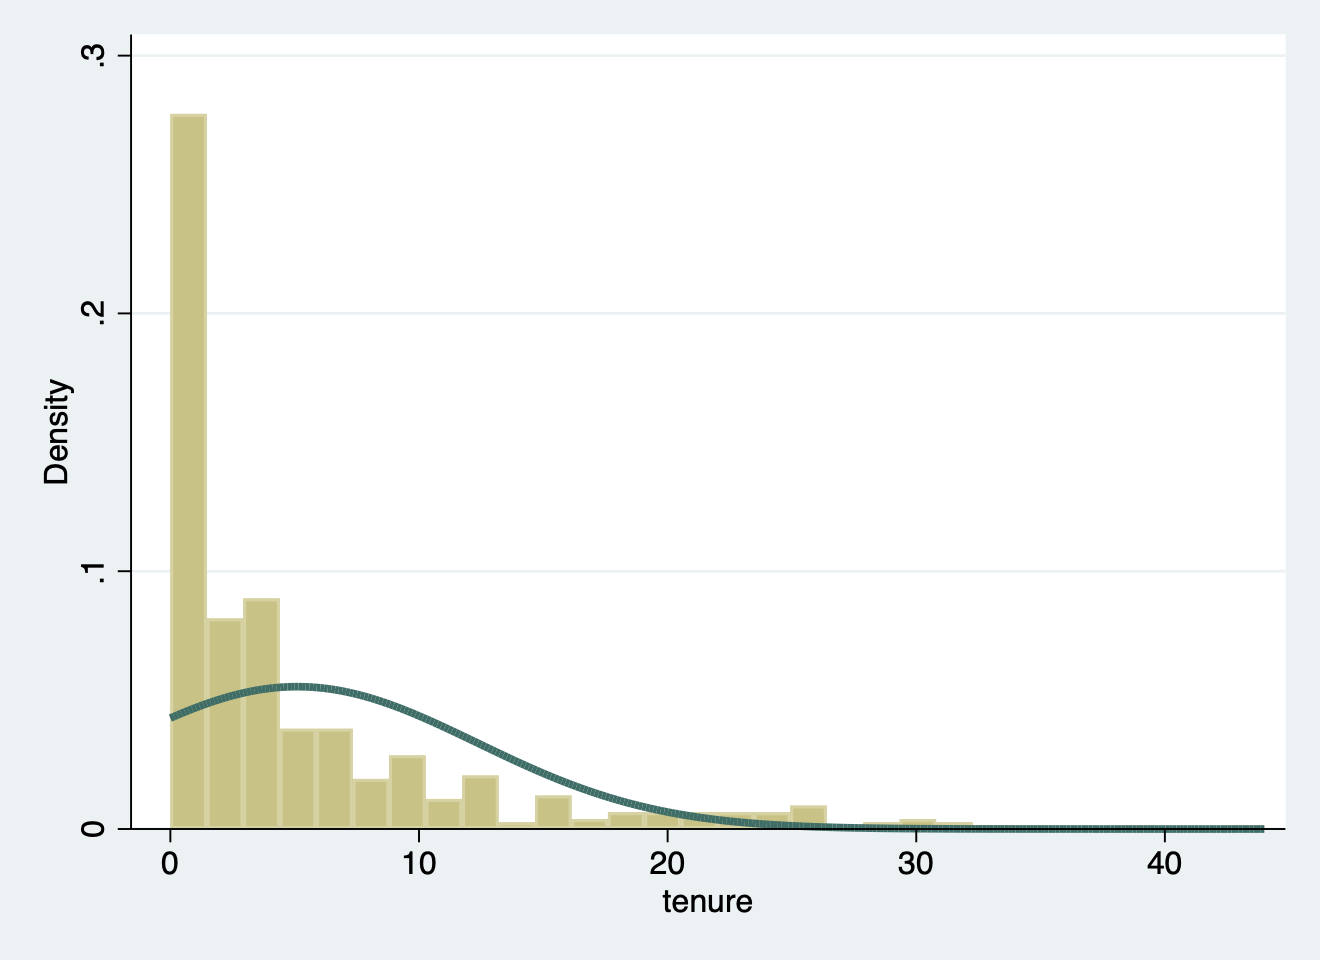
\includegraphics[scale=.3]{PLOT_7.png}
\end{center}
\end{block}
\end{frame}

\begin{frame}{Application STATA}
\begin{block}{Régression linéaire simple}
\begin{equation}
wage = \beta_0 + \beta_1 educ  + \epsilon
\end{equation}
\begin{equation}
wage = \beta_0 + \beta_1 exper  + \epsilon
\end{equation}
\begin{equation}
wage = \beta_0 + \beta_1 tenure  + \epsilon
\end{equation}
\end{block}
\begin{block}{Régression linéaire multiple}
\begin{equation}
wage = \beta_0 + \beta_1 educ +\beta_2 exper + \beta_3 tenure  + \epsilon
\end{equation}
\end{block}
\end{frame}

\begin{frame}{Application STATA}
\begin{block}{Code 11: $wage = \beta_0 + \beta_1 educ  + \epsilon$}
\textbf{reg wage educ}
\end{block}

\begin{block}{Output 11:}
\begin{center}
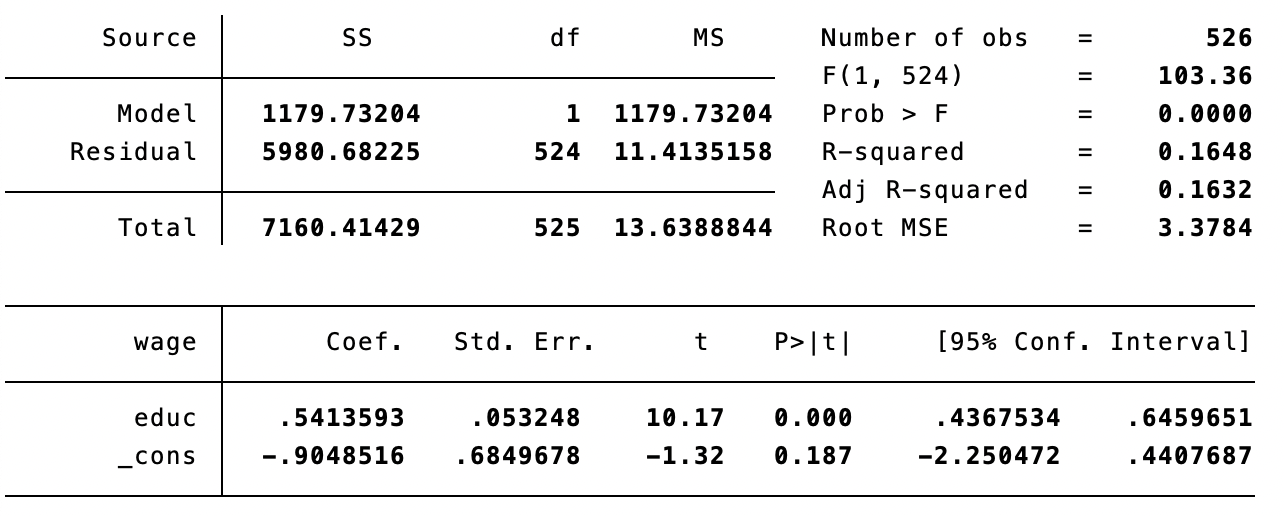
\includegraphics[scale=.5]{REG1.png}
\end{center}
\end{block}
\end{frame}


\begin{frame}{Application STATA}
\begin{block}{Analyse: $wage = \beta_0 + \beta_1 educ  + \epsilon$}
\begin{itemize}
\item Avec un $R^2$ de 0.1648, le nombre d’années d’éducation d'un salarié semble expliquer environ 16\% des variations dans le salaire de ce dernier, et ce en moyenne.
\item La p-value du T-test pour le coefficient de la variable educ est de 0.000, ce qui implique que le coefficient est significativement différent de zéro. (À un seuil de 5\%)
\item Avec un coefficient estimé de 0.54 pour la variable educ, on peut comprendre qu’en moyenne, une année d’éducation additionnelle amène une augmentation du salaire horaire de 0.54.
\end{itemize}
\end{block}
\end{frame}





\begin{frame}{Application STATA}
\begin{block}{Code 12: $wage = \beta_0 + \beta_1 exper  + \epsilon$}
\textbf{reg wage exper}
\end{block}

\begin{block}{Output 12:}
\begin{center}
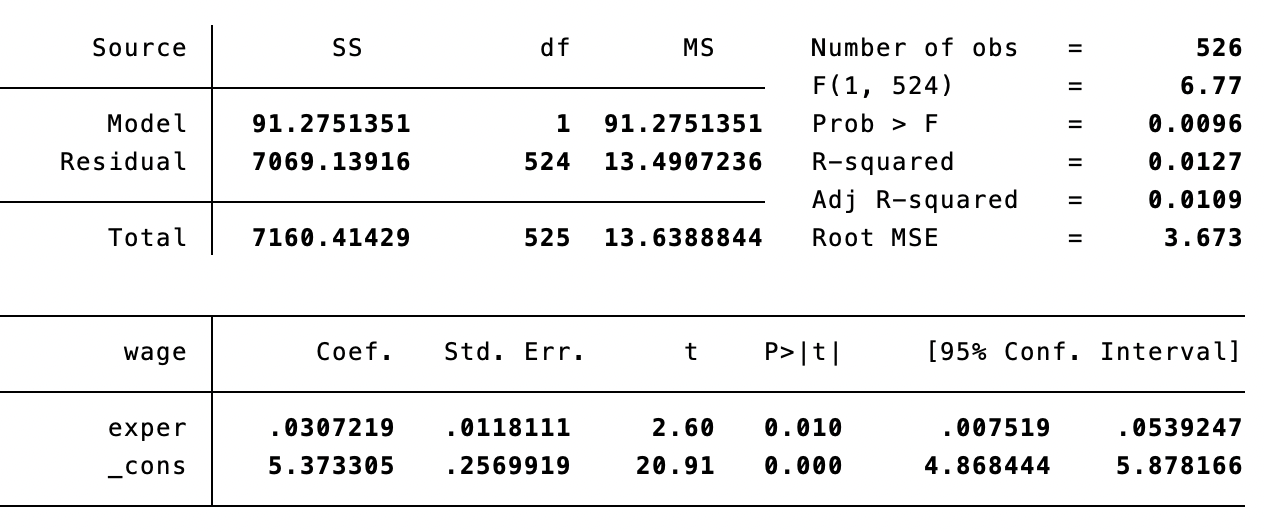
\includegraphics[scale=.5]{REG2.png}
\end{center}
\end{block}
\end{frame}

\begin{frame}{Application STATA}
\begin{block}{Analyse: $wage = \beta_0 + \beta_1 exper  + \epsilon$}
\begin{itemize}
\item Avec un $R^2$ de 0.0127, le nombre d’années d’expérience d'un salarié semble expliquer environ 1\% des variations dans le salaire de ce dernier, et ce en moyenne.
\item La p-value du T-test pour le coefficient de la variable exper est de 0.01, ce qui implique que le coefficient est significativement différent de zéro. (À un seuil de 5\%)
\item Avec un coefficient estimé de 0.0307 pour la variable exper, on peut comprendre qu’en moyenne, une année d’expérience additionnelle amène une augmentation du salaire horaire de 0.0307.
\end{itemize}
\end{block}
\end{frame}
\begin{frame}{Application STATA}
\begin{block}{Code 13: $wage = \beta_0 + \beta_1 tenure  + \epsilon$}
\textbf{reg wage tenure}
\end{block}

\begin{block}{Output 13:}
\begin{center}
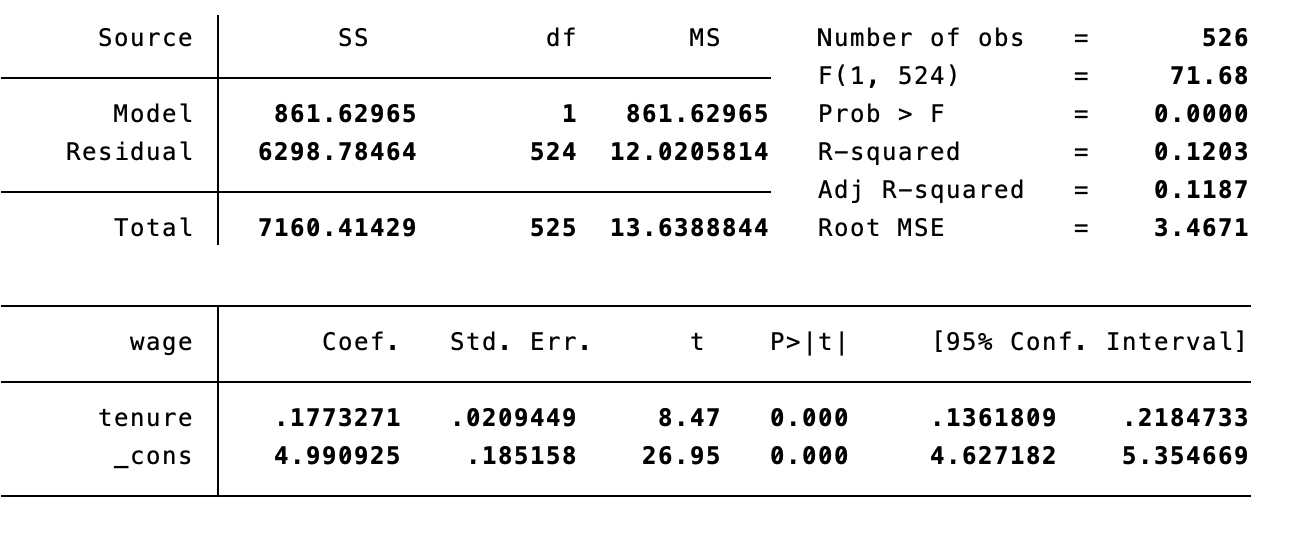
\includegraphics[scale=.5]{REG3.png}
\end{center}
\end{block}
\end{frame}


\begin{frame}{Application STATA}
\begin{block}{Analyse: $wage = \beta_0 + \beta_1 tenure  + \epsilon$}
\begin{itemize}
\item Avec un $R^2$ de 0.1203, le nombre d’années chez l'employeur actuel d'un salarié semble expliquer environ 12\% des variations dans le salaire de ce dernier, et ce en moyenne.
\item La p-value du T-test pour le coefficient de la variable tenure est de 0.000, ce qui implique que le coefficient est significativement différent de zéro. (À un seuil de 5\%)
\item Avec un coefficient estimé de 0.177 pour la variable tenure, on peut comprendre qu’en moyenne, une année de plus chez l'employeur actuel amène une augmentation du salaire horaire de 0.177.
\end{itemize}
\end{block}
\end{frame}

\begin{frame}{Application STATA}
\begin{block}{Code 14: $wage = \beta_0 + \beta_1 educ +\beta_2 exper + \beta_3 tenure  + \epsilon$}
\textbf{reg wage educ exper tenure}
\end{block}

\begin{block}{Output 14:}
\begin{center}
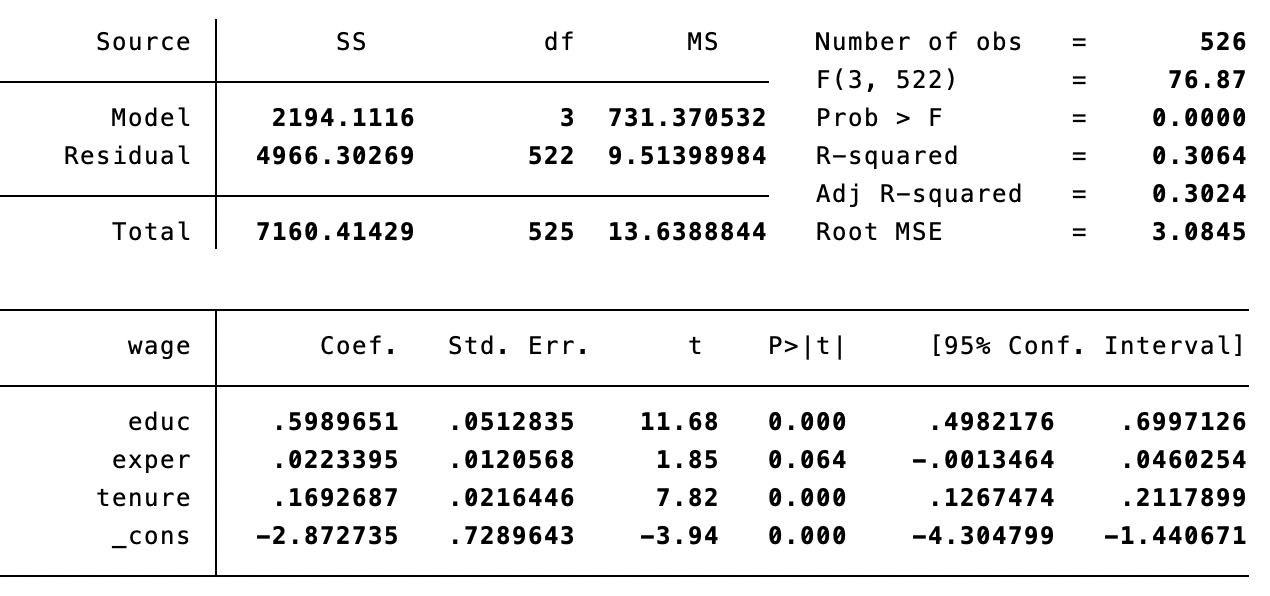
\includegraphics[scale=.5]{REG4.png}
\end{center}
\end{block}
\end{frame}

\begin{frame}{Application STATA}
\begin{block}{Analyse: $wage = \beta_0 + \beta_1 educ +\beta_2 exper + \beta_3 tenure  + \epsilon$}
\begin{itemize}
\item Avec un $R^2$ de 0.3064, les trois variables combinées ensemble semblent expliquer environ 31\% des variations dans le salaire de ce dernier, et ce en moyenne.
\item De plus, avec un $R^2$ ajusté de 0.3024 (relativement proche du $R^2$ standard), l'ajout de variables explicatives semble justifier étant donné que la valeur du $R^2$ ajusté ne semble pas avoir diminuer grandement par rapport au $R^2$ standard, suite à la pénalité pour l'ajout de variables explicatives dans le $R^2$ ajusté.
\item La p-value du F-test est de 0.000, ce qui implique que nous pouvons rejeter l'hypothèse nulle que tous les coefficients sont conjointement non significatifs. 
\end{itemize}
\end{block}
\end{frame}

\begin{frame}{Détails sur le T-test}

\begin{itemize}
\item Dans le T-test que nous venons de faire, nous avons utilisé la P-value pour vérifier si le coefficient est significativement différent de 0.
\item En effet si cette P-value est inférieur à 0.05, on rejette l’hypothèse nulle que le coefficient est pas significativement différent de 0.
\item Afin de bien comprendre comment le T-test fonctionne, il est important de bien faire l’analyse sans utiliser la P-value.
\item Nous allons reprendre la dernière régression que nous venons d’analyser, soit celle avec toutes les variables explicatives incluses.
\end{itemize}

\end{frame}

\begin{frame}{Détails sur le T-test}
\textbf{Test de Student:}
\begin{block}{Two-tailed test}
\begin{itemize}
\item Hypothèse nulle est la non-significativité du coefficient de régression
\item Hypothèses:
\begin{itemize}
\item $H_0:$ $\beta_k=0$ $\rightarrow$ \textbf{Hypothèse nule}
\item $H_1:$ $\beta_k \neq 0$ $\rightarrow$ \textbf{Hypothèse alternative}
\end{itemize}
\item Règle de décision:
Rejeter $H_0$ si:
\begin{align*}
t=\frac{\mid \hat{\beta}_k-\beta_0 \mid}{SE_{\hat{\beta}_k}} > t_{n-k,\alpha/2}
\end{align*}
\begin{itemize}
\item Ou $\beta_0$ est la valeur du coefficient sous l'hypothèse nulle, soit 0
\item $SE_{\hat{\beta}_k}$ est l'écart-type associé à l'estimation de $\hat{\beta}_k$
\end{itemize}
\end{itemize}
\end{block}

\end{frame}

\begin{frame}{Détails sur le T-test}

\begin{itemize}
\item Le Modèle de régression:
\begin{align*}
wage = \beta_0 + \beta_1 educ +\beta_2 exper + \beta_3 tenure  + \epsilon
\end{align*}
\item Afin de pouvoir faire la comparaison de notre statistique T, nous devons obtenir une valeur critique à un seuil de 5\%, soit 
\begin{align*}
t_{n-k,\alpha/2}
\end{align*}
\item Sachant que nous avons $n=526$ observations et $k=3$ variables explicatives, nous devrons trouve la valeur critique:
\begin{align*}
t_{526-3,0.05/2}=t_{523,0.025}
\end{align*}

\end{itemize}

\end{frame}

\begin{frame}{Détails sur le T-test}

\begin{itemize}
\item Nous allons maintenant aller regarder dans une table statistique appelée \textbf{T-table} afin de trouver notre valeur critique.
\item Au niveau de la significativité, on prendra la colonne avec une valeur: 
\begin{itemize}
\item $\alpha= 0.025$ pour le \textbf{One-tail test}
\item $\alpha= 0.05$ pour le \textbf{Two-tail test}
\end{itemize}
\item Pour ce qui est du nombre de degrés de liberté, nous avons $df=523$, cependant la table ne fournit pas nécessairement une valeur pour tous les df possibles.
\begin{itemize}
\item Dans la table qui va suivre, nous avons seulement $df=100$ et $df=1000$ de dispo, nous allons donc prendre $df=1000$ par sécurité.
\end{itemize}
\end{itemize}

\end{frame}

\begin{frame}{Détails sur le T-test}
\begin{center}
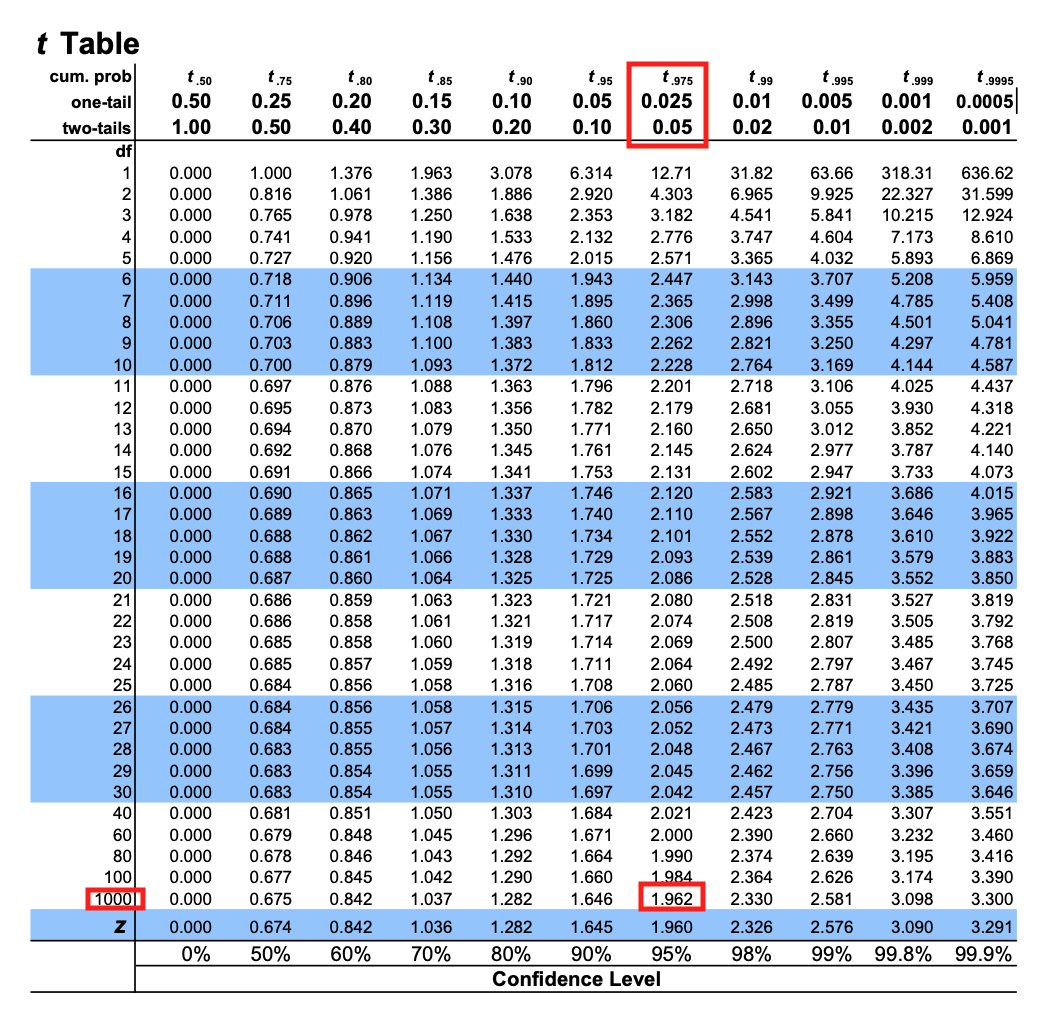
\includegraphics[scale=.4]{tstat}
\end{center}
\end{frame}

\begin{frame}{Détails sur le T-test}
\begin{itemize}
\item Notre valeur critique est de $t_{526-3,0.05/2}=t_{523,0.025}=1.962$
\item Pour le coefficient $\beta_1$ attaché à la variable \textbf{educ}:
\begin{align*}
t=\frac{\mid 0.5989651-0 \mid}{0.0512835} = 11.69 > 1.962
\end{align*}
\begin{itemize}
\item $t=11.69$ est plus grand que la valeur critique $t_{523,0.025}=1.962$, alors on peut rejetter l'hypothèse nulle et conclure que $\hat{\beta}_1$ est significativement différent de 0, à un seuil de 5\%.
\end{itemize}
\end{itemize}
\end{frame}

\begin{frame}{Détails sur le T-test}
\begin{itemize}
\item Pour le coefficient $\beta_2$ attaché à la variable \textbf{exper}:
\begin{align*}
t=\frac{\mid 0.0223395-0 \mid}{0.0120568} = 1.85 < 1.962
\end{align*}
\begin{itemize}
\item $t=1.85$ est plus petit que la valeur critique $t_{523,0.025}=1.962$, alors on ne peut pas rejetter l'hypothèse nulle. $\hat{\beta}_2$ n'est pas significativement différent de 0, à un seuil de 5\%.
\end{itemize}
\end{itemize}
\end{frame}

\begin{frame}{Détails sur le T-test}
\begin{itemize}

\item Pour le coefficient $\beta_3$ attaché à la variable \textbf{tenure}:
\begin{align*}
t=\frac{\mid 0.1692687-0 \mid}{0.0216446} = 7.82 > 1.962
\end{align*}
\begin{itemize}
\item $t=7.82$ est plus grand que la valeur critique $t_{523,0.025}=1.962$, alors on peut rejetter l'hypothèse nulle et conclure que $\hat{\beta}_3$ est significativement différent de 0, à un seuil de 5\%.
\end{itemize}
\end{itemize}
\end{frame}


\begin{frame}{Détails sur le F-test}
\begin{itemize}
\item Comme pour le T-test, on veut également effectuer le F-test sans la P-value.
\end{itemize}
\textbf{F-test (significativité conjointe)}
\begin{block}{Hypothèses:}
\begin{itemize}
\item $H_O:$ $\beta_2 =0$ et/ou $\beta_3 = 0$ et/ou $...$ et/ou $\beta_k=0$
\item $H_1:$ $\beta_2 \neq 0$ et $\beta_3 \neq 0$ et $...$ et/ou $\beta_k \neq 0$
\end{itemize}
\end{block}
\begin{block}{Statistique de test:}
\begin{align*}
F=\frac{MS_{group}}{MS_{error}}>F(q,t-k;\alpha)
\end{align*}
Sachant
\begin{itemize}
\item $MS_{group}=\frac{SS_{group}}{df_{group}}$
\item $MS_{error}=\frac{SS_{error}}{df_{error}}$
\end{itemize}
\end{block}
\end{frame}

\begin{frame}{Détails sur le F-test}
\begin{itemize}
\item On rejette $H_0$ si la statistique $F$ est supérieur à la valeur critique $F(q,t-k;\alpha)$.
\item Dans le cas qui nous concerne, nous avons 4 coefficients (k=4), soit $\beta_0, \beta_1, \beta_2$ et $\beta_3$
\item $q=k-1=4-1=3= df_{group}$
\item $t-k=526-4=522= df_{error}$
\item On pose un seuil de significativité de $\alpha=0.05$
\item La valeur critique sera représenté par $F(3,522;0.05)$
\item Nous allons maintenant regarder dans la table suivante la valeur critique $F(3,522;0.05)$
\end{itemize}
\end{frame}

\begin{frame}{Détails sur le F-test}
\begin{center}
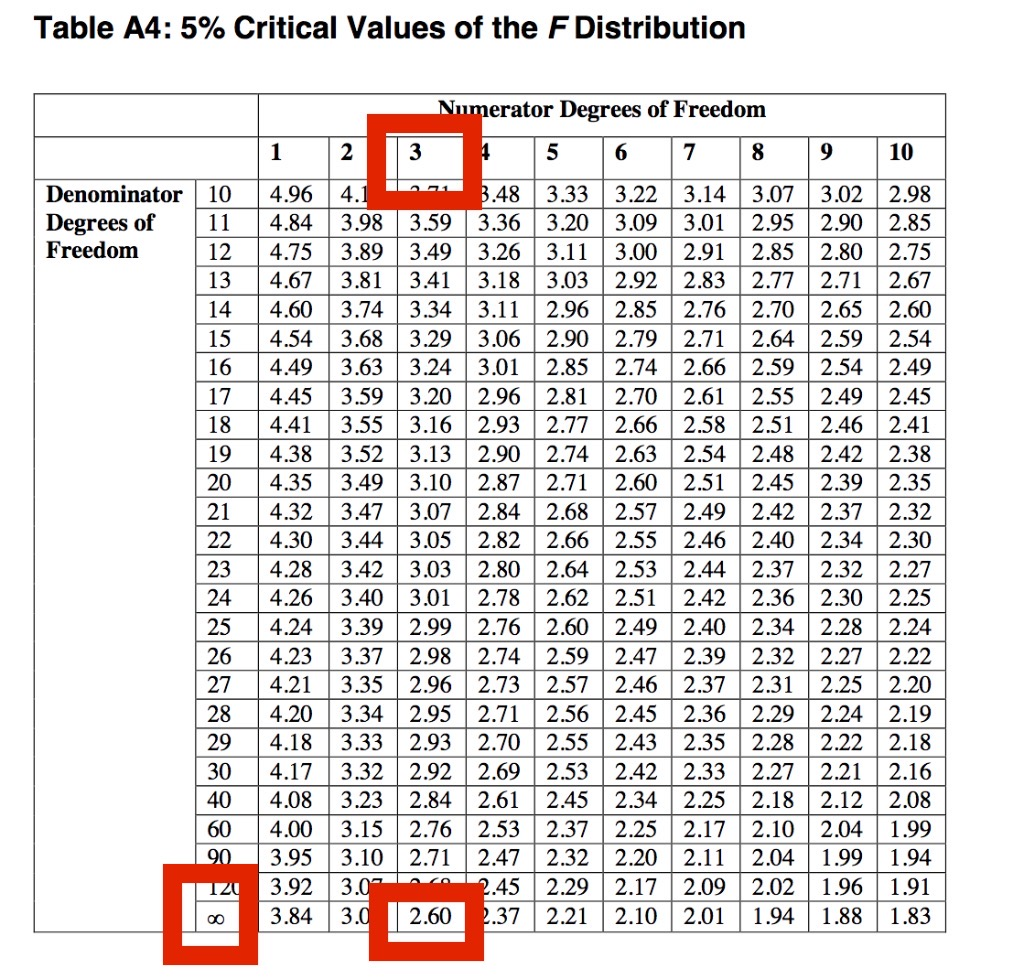
\includegraphics[scale=.2]{ftable}
\end{center}
\end{frame}

\begin{frame}{Détails sur le F-test}
\begin{itemize}
\item La valeur de la statistique F est:
\begin{align*}
F(3,522;0.05)=2.60
\end{align*}
\item Voici maintenant le test:
\begin{align*}
F=\frac{\frac{SS_{group}}{df_{group}}}{\frac{SS_{error}}{df_{error}}}>F(q,t-k;\alpha)
\end{align*}
\begin{align*}
F=\frac{\frac{2194.1116}{3}}{\frac{4966.30269}{522}}=76.87>2.60
\end{align*}
\end{itemize}
\end{frame}


\begin{frame}{Détails sur le F-test}
\begin{itemize}
\item On rejette l'hypothèse nulle étant donné que la statistique $F=76.87$ est supérieur à la valeur critique $F(3,522;0.05)=2.60$.
\item On rejette donc l'hypothèse que tous les coefficients sont conjointement tous égaux à 0.
\item En d'autres mots, au moins un coefficient dans cette régression est significativement différent de 0.
\end{itemize}
\end{frame}


\begin{frame}{Application STATA}

\begin{block}{Code 15: Générer les résidus de la régression}
\textbf{reg wage educ exper tenure}\\
\textbf{predict resid, residuals}
\end{block}
\begin{itemize}
\item Sans faire une analyse détaillée des résidus, nous allons créer une variable représentant les résidus de notre régression.
\item Afin de faire l'analyse, nous allons produire un histogramme de nos résidus et un nuage de points avec les résidus en axe des Y et la variable \textbf{wage} en axe des X.
\end{itemize}
\end{frame}

\begin{frame}{Application STATA}

\begin{block}{Code 16: Histogramme des résidus}
\textbf{histogram resid, bin(50) normal}
\end{block}

\begin{block}{Output 16:}
\begin{center}
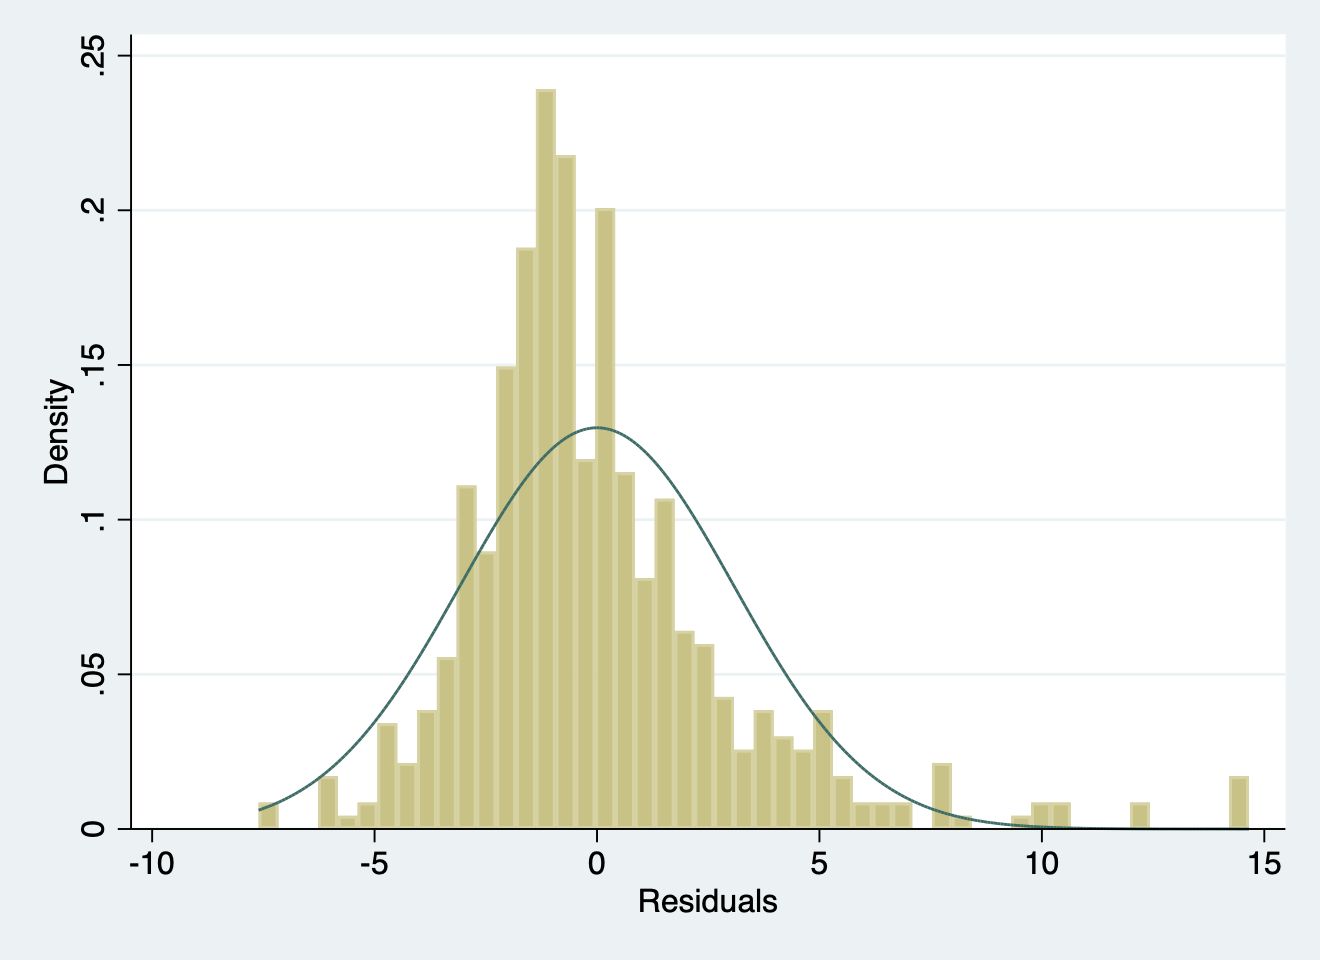
\includegraphics[scale=.3]{resid.png}
\end{center}
\end{block}

\end{frame}



\begin{frame}{Application STATA}

\begin{block}{Code 17: Nuage de points des résidus}
\textbf{twoway (scatter red wage)}
\end{block}

\begin{block}{Output 17:}
\begin{center}
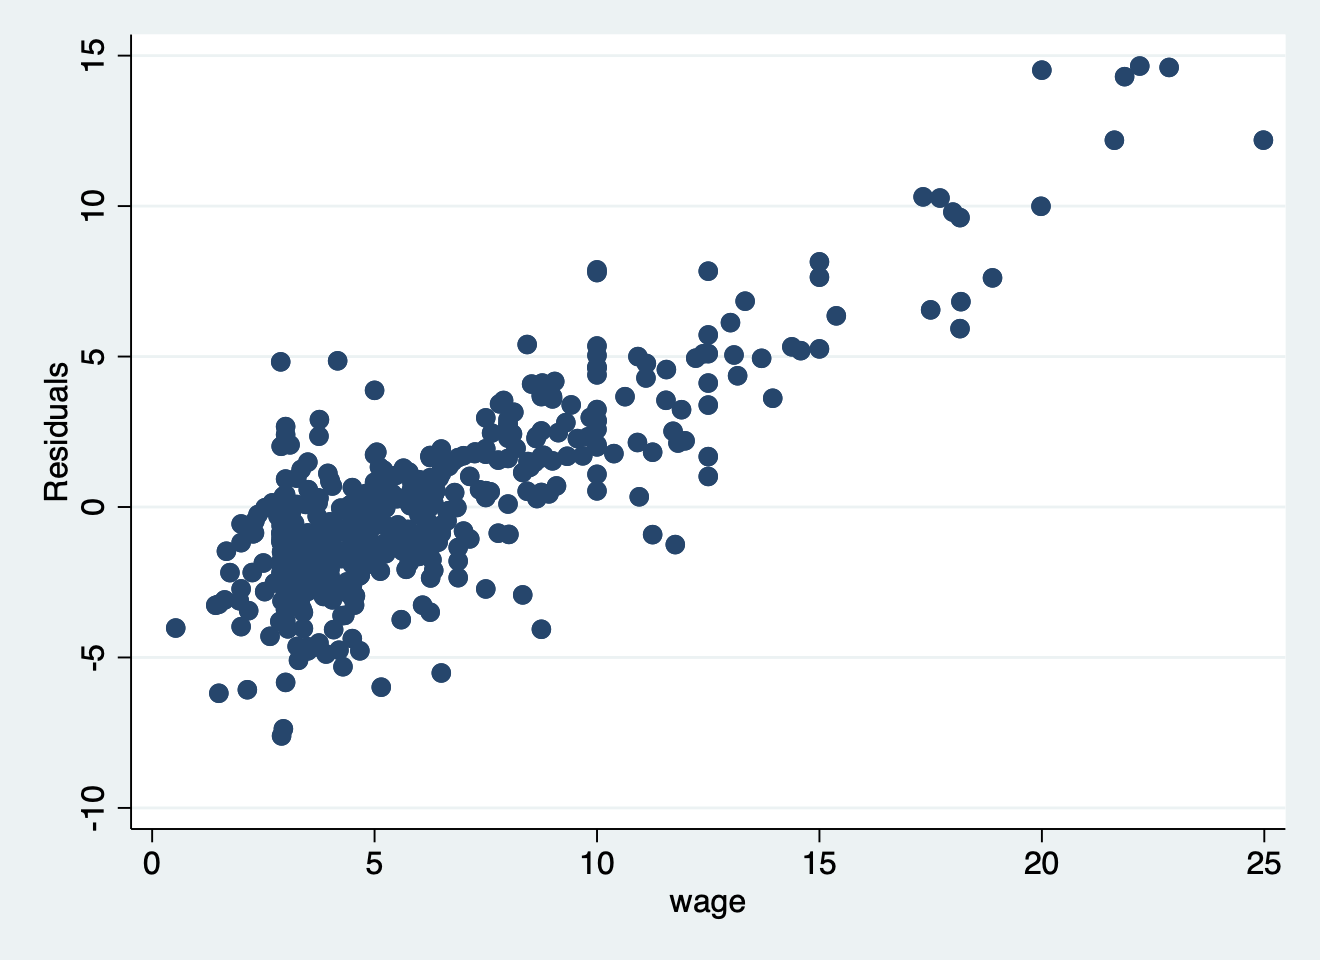
\includegraphics[scale=.3]{scatter_resid.png}
\end{center}
\end{block}

\end{frame}


\begin{frame}{Application STATA}

\begin{block}{Analyse des résidus}
\begin{itemize}
\item Comme caractéristiques souhaitez pour nos résidus, nous souhaitons qu’il ressemble à une loi normale et qu’il n’ait pas de \textbf{patterns} entre ce résidu et la variable \textbf{wage}
\item Au niveau de l’histogramme des résidus, on peut voir que sans être parfaits les résidus prennent la forme d’une cloche. 
\item Il semble y avoir plus de résidus au niveau du centre (x=0), que ce qui est prévu par la loi normale.
\item Au niveau du nuage de point, nous avons un problème majeur, il y a clairement une relation entre notre résidu et la variable \textbf{wage}.
\end{itemize}
\end{block}

\end{frame}


\end{document}